\documentclass[11pt]{article}
\usepackage[margin=1in]{geometry}
\usepackage{amsmath,amssymb,amsthm,booktabs,graphicx,hyperref}
\hypersetup{colorlinks=true,linkcolor=blue,citecolor=blue,urlcolor=blue}
\newtheorem{theorem}{Theorem}
\newtheorem{lemma}{Lemma}
\newcommand{\Tr}{\operatorname{Tr}}
\newcommand{\M}{\mathcal M}

\title{All bivariate quartic tracial moment sequences\\admit size-two representations}
\author{Run \texttt{fa\_banach\_001}, lane 1 (GPT5.6)}
\date{11 August 2026}

\begin{document}
\maketitle

\begin{center}
\fbox{\parbox{0.9\textwidth}{\textbf{Status: candidate full result, likely valid.}
Every representable bivariate quartic real tracial moment sequence has a
representing measure whose atoms have size at most two.}}
\end{center}

\section{Source and target}

For a normalized real tracial sequence
$\beta=(\beta_w)_{|w|\leq4}$ in two noncommuting self-adjoint variables,
a representing measure is a finite convex combination
\[
 \beta_w=\sum_i\lambda_i\Tr\bigl(w(A_i,B_i)\bigr),
 \qquad \lambda_i>0,\quad \sum_i\lambda_i=1,
\]
where $A_i,B_i$ are real symmetric matrices of a common size within each
atom and $\Tr$ is normalized trace.  Its order-two moment matrix $\M_2$ is
the $7\times7$ matrix indexed by
$1,X,Y,X^2,XY,YX,Y^2$ \cite{BZ17}.

Bhardwaj--Zalar prove that atoms of size at most two suffice in every case
except a rank-six normal form satisfying $Y^2=1$ \cite[pp.~3--4]{BZ17}.
Their page-spanning statement is reproduced below.

\begin{figure}[ht]
\centering
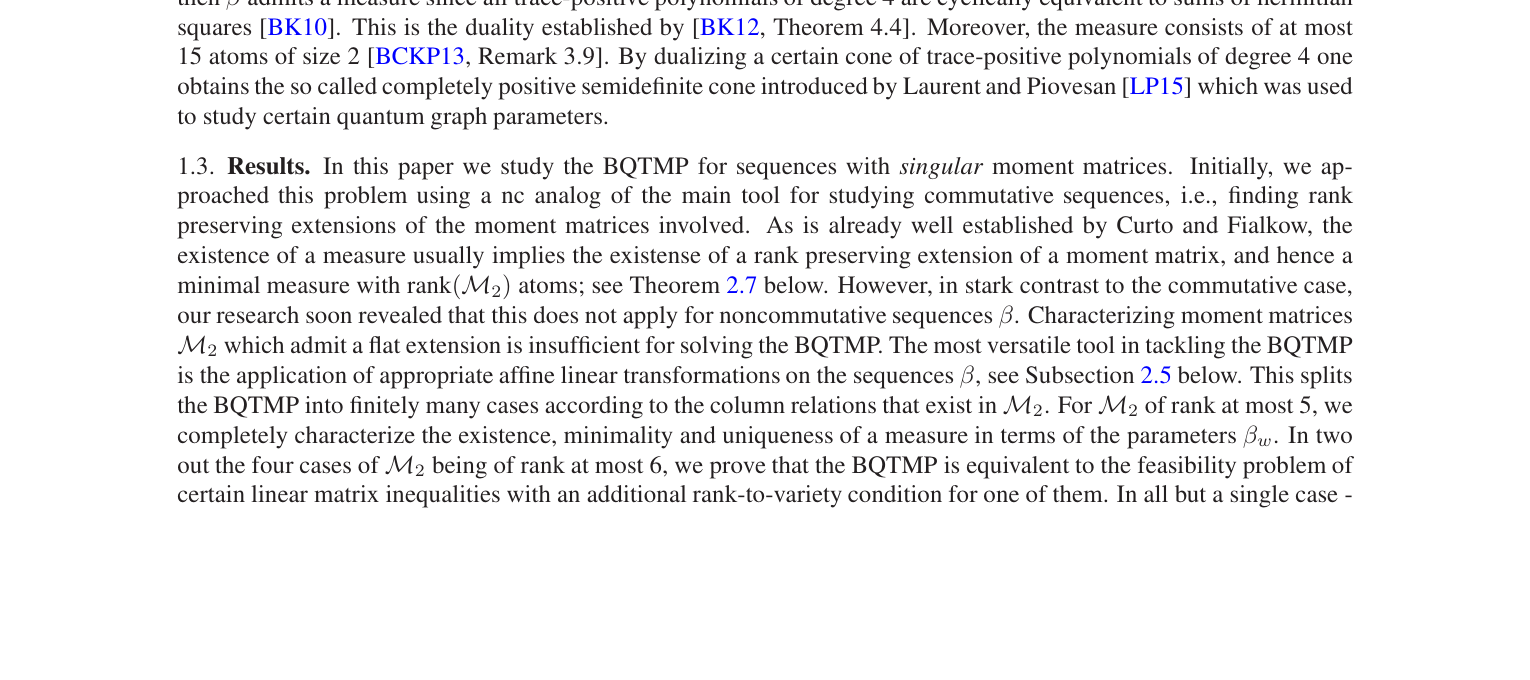
\includegraphics[width=\textwidth]{figures/source_rank_cases_part1.png}
\vspace{2mm}
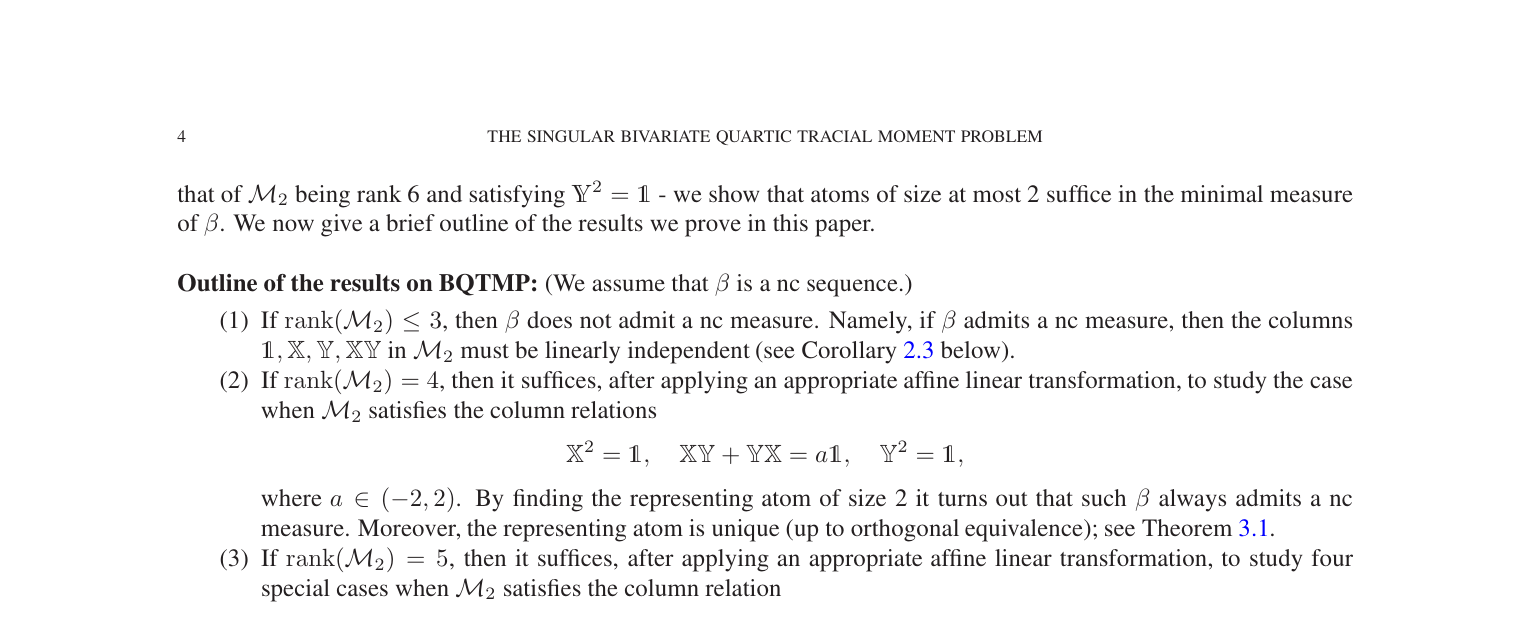
\includegraphics[width=\textwidth]{figures/source_rank_cases_part2.png}
\caption{The source identifies a single missing size-two case: rank six with
$Y^2=1$ (arXiv:1611.00494, pp.~3--4).}
\end{figure}

The later paper \cite{BZ20} formulates the missing $Y^2=1$ assertion as its
Conjecture~1.  The previous full packet \cite{PriorPacket} proves that
conjecture for arbitrary finite atom sizes, not merely for size-three atoms.
The present note records the resulting all-rank conclusion.

\clearpage
\section{Proof intuition}

There are only seven rank possibilities for $\M_2$.  The commutative case is
already scalar: equality of the two cyclic fourth moments forces the
commutator of every atom to vanish.  For a noncommutative sequence the source
forces rank at least four.  Rank seven is the positive-definite theorem;
ranks four and five are covered constructively in the source.  At rank six,
an invertible affine change of $X,Y$ gives one of four quadratic normal forms.
The source covers the first three, and the earlier GPT5.6 theorem covers the
fourth, $Y^2=1$.  Inverting the affine change does not alter matrix size.

\section{Two elementary reductions}

\begin{lemma}[The commutative case is scalar]\label{lem:comm}
If a representable quartic tracial sequence satisfies
$\beta_{X^2Y^2}=\beta_{XYXY}$, then it has a representing measure using only
scalar atoms.
\end{lemma}

\begin{proof}
For real symmetric matrices $A,B$, cyclicity of normalized trace gives
\begin{align*}
 \Tr(A^2B^2)-\Tr(ABAB)
 &=\frac12\Tr\bigl((AB-BA)^T(AB-BA)\bigr)\geq0.
\end{align*}
Apply this identity to every atom of a representing measure and average with
the positive densities.  Equality of the two moments forces every summand on
the right to vanish.  Thus $A_iB_i=B_iA_i$ for every atom.  Each real symmetric
commuting pair is simultaneously orthogonally diagonalizable.  Splitting its
normalized trace over the joint eigenvectors replaces it by scalar atoms and
preserves all moments (indeed, all word moments).
\end{proof}

\begin{lemma}[Affine normalization preserves atom size]\label{lem:affine}
Let
\[
 \widetilde X=a_0+a_1X+a_2Y,\qquad
 \widetilde Y=b_0+b_1X+b_2Y
\]
with invertible linear part.  A quartic sequence has a representation by
atoms of size at most two if and only if its transformed sequence does.
\end{lemma}

\begin{proof}
Apply the displayed affine formulas to each pair $(A_i,B_i)$, inserting the
identity matrix for the constant terms.  The matrix size is unchanged.  The
inverse affine formulas give the converse.
\end{proof}

\section{Full theorem}

\begin{theorem}\label{thm:main}
Every normalized bivariate quartic real tracial moment sequence that admits a
representing measure by finite real symmetric matrix pairs admits a
representing measure whose atoms all have size at most two.
\end{theorem}

\begin{proof}
Let $r=\operatorname{rank}\M_2\leq7$.  Lemma~\ref{lem:comm} settles the
commutative case, so suppose the sequence is noncommutative.

The source proves that $1,X,Y,XY$ are linearly independent in this case
\cite[Corollary~2.3]{BZ17}; hence $r\geq4$.

If $r=7$, then $\M_2$ is positive definite.  The positive-definite quartic
theorem gives a representing measure with at most fifteen atoms, all of size
two \cite[p.~3, citing Remark~3.9 of BCKP13]{BZ17}.

If $r=4$, Theorem~3.1 of \cite{BZ17} constructs a size-two atom after an
invertible affine normalization.  Lemma~\ref{lem:affine} transfers it back.
If $r=5$, the four normal forms are handled by Theorems~6.5, 6.8, 6.11 and
6.14 of \cite{BZ17}; their measures use scalar atoms and one size-two atom.

It remains that $r=6$.  Proposition~4.1(2) of \cite{BZ17}, followed by an
invertible affine change, reduces the sequence to one of
\[
 X^2+Y^2=1,\qquad XY+YX=0,\qquad Y^2-X^2=1,\qquad Y^2=1.
\]
The source proves that the first three normal forms have minimal measures with
atoms of size at most two \cite[p.~4]{BZ17}; see the evidence crop below.
\begin{center}
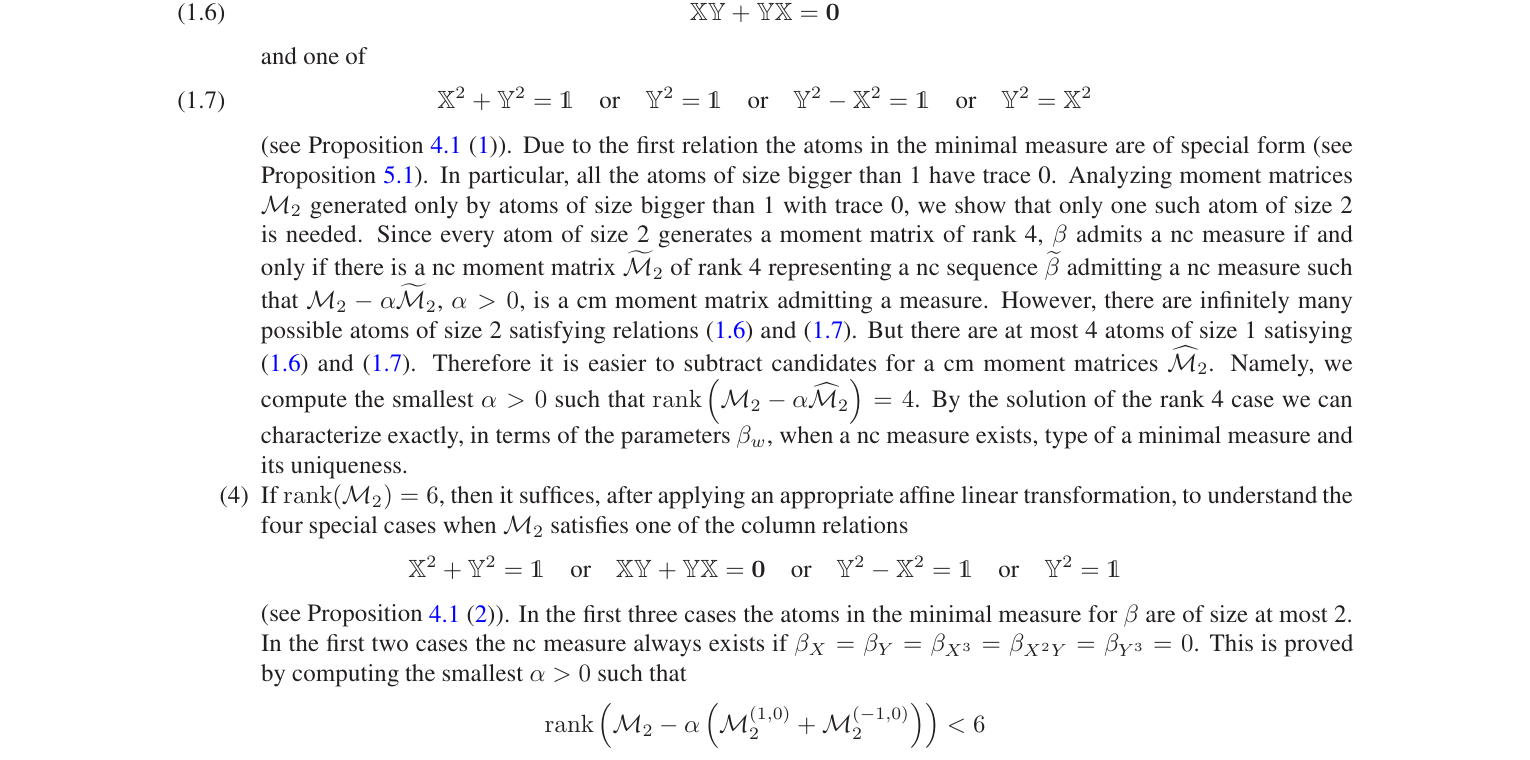
\includegraphics[width=\textwidth]{figures/source_rank6_normal_forms.png}
\end{center}
For the remaining form $Y^2=1$, Theorem~1 of the prior full packet
\cite{PriorPacket} proves that every arbitrary representing measure can be
replaced by one of type $(m,1)$: one size-two atom and at most four scalar
atoms.  Finally use Lemma~\ref{lem:affine} to invert the normalization.

This exhausts $r=4,5,6,7$ and completes the proof.
\end{proof}

\section{Verification and limitations}

The reusable script \texttt{code/verify\_rank\_exhaustion.py} checks the
commutator identity on 2,000 seeded random symmetric pairs of sizes one
through nine and mechanically verifies that ranks one through seven and all
four rank-six normal forms have an assigned branch.  It is a regression test,
not evidence for the cited source theorems.

This theorem is about degree-four moments in exactly two self-adjoint
variables.  It does not claim a size-two bound for higher truncation degree,
more variables, complex non-self-adjoint variables, or prescribed supports.

The broad conjecture appears in commented source material of
arXiv:1611.00494 rather than as a numbered statement in the final PDF.  The
published PDF nevertheless explicitly says that size two is proved ``in all
but a single case'' and names that case as rank six with $Y^2=1$.  The later
paper \cite{BZ20} explicitly promotes that missing case to Conjecture~1.

\section{Novelty check and review recommendation}

On 11 August 2026 we searched the run registry and solution/attempt/proof-gap
indexes for arXiv:1611.00494, the exact title, ``bivariate quartic tracial
moment'', ``atoms of size at most 2'', and the $Y^2=1$ normal form.  We also
searched primary arXiv results for the exact conjecture and close atom-size
phrases.  We found \cite{BZ17}, \cite{BZ20}, the earlier run packet
\cite{PriorPacket}, and no later paper stating the all-rank synthesis.
Novelty confidence is moderate because the conclusion is a short but
apparently unrecorded corollary of those inputs.

Human review should focus on two interfaces: that Proposition~4.1 uses an
invertible affine normalization, and that the source's “first three cases” are
exactly the three displayed rank-six forms other than $Y^2=1$.  The last form
is the exact scope of Theorem~1 in \cite{PriorPacket}.

\begin{thebibliography}{9}
\bibitem{BZ17}
A. Bhardwaj and A. Zalar,
\emph{The singular bivariate quartic tracial moment problem},
arXiv:1611.00494, 2017.

\bibitem{BZ20}
A. Bhardwaj and A. Zalar,
\emph{The tracial moment problem on quadratic varieties},
arXiv:2001.11614; J. Math. Anal. Appl. 498 (2021), 124936.

\bibitem{PriorPacket}
Run \texttt{fa\_banach\_001},
\emph{One size-two atom suffices for the quartic tracial moment problem on
$Y^2=1$}, full solution packet for arXiv:2001.11614, GPT5.6, 2026.
\end{thebibliography}

\end{document}

